\chapter{Ergebnisse}
\label{ch:ergebnis}

	\section{Latenz}
	\label{sec:ergebnis:latenz}
	
		\subsection{Sicherheitslevel 1}
		\label{subsec:ergebnis:latenz:sl1}
		
		Zwischen der hinzugefügten Latenz pro Paket und der Dauer des Handshakes besteht ein nahezu perfekter 				linearer Zusammenhang (vgl. Abbildung \ref{fig:ergebnis:latenz:sl1}. Dabei liegt die Performanz bei den 		unterschiedlichen betrachteten Algorithmen des Sicherheitslevel 1 so eng beieinander, dass die 					entstehenden Graphen dicht aneinander angrenzen und einander teils verdecken.\\
		
		\begin{figure}[htbp]
			\centering
			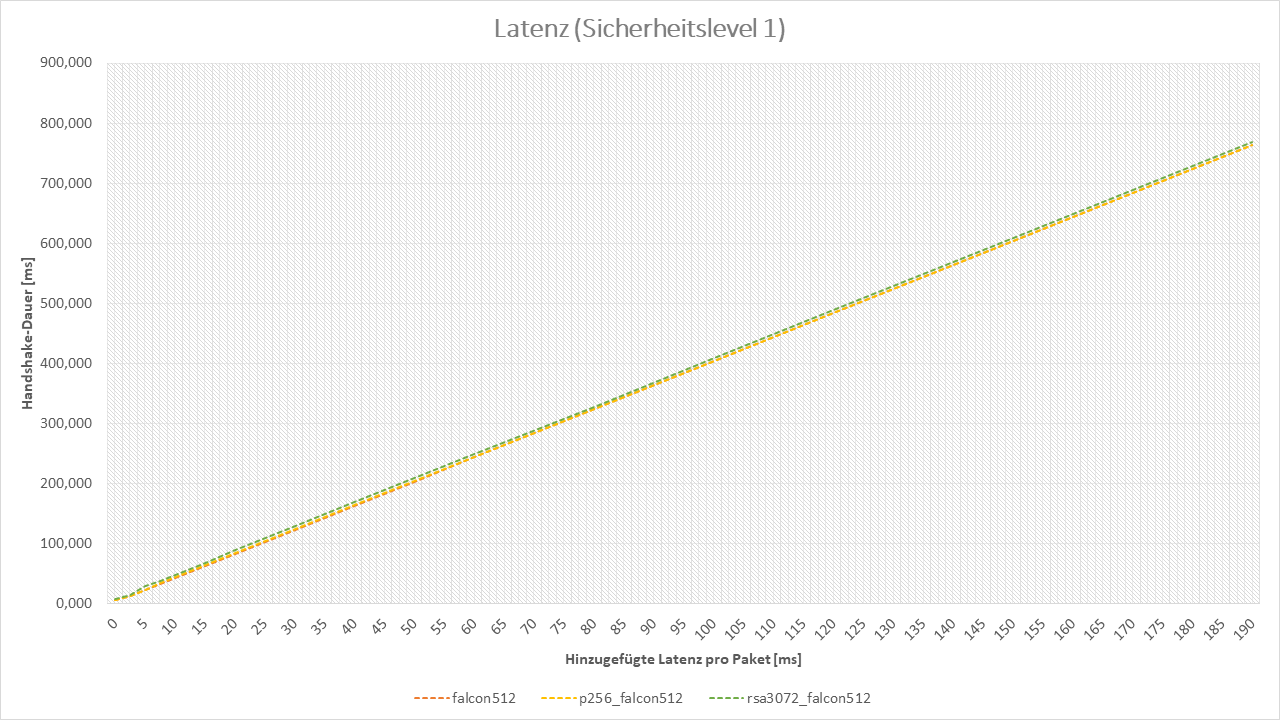
\includegraphics[width=\textwidth]{../auswertung/latenz_sl1.png}
			\caption{Auswertung der Variation der Latenz bei Algorithmen mit Sicherheitslevel 1}
			\label{fig:ergebnis:latenz:sl1}
		\end{figure}
		
		Dies ist insofern erklärbar, dass die Latenz technisch eine Verzögerung ist, die zu jedem einzelnen 				Paket hinzugefügt wird. Eine höhere Verzögerung in jedem einzelnen von n Paketen bewirkt eine n-mal 				höhere Gesamtverzögerung. Entsprechend entsteht ein linearer Zusammenhang.\\
		
		Es kann eine leicht bessere Performanz von Falcon-512 mit P-256 sowie eine leicht schlechtere 						Performanz von Falcon-512 mit RSA-3.072 gegenüber dem reinen Falcon-512-Algorithmus beobachtet werden. Falcon-512 mit RSA-3.072 hatte dabei eine maximale Handshake-Dauer von 767,868ms. 			Dies bewegt sich jedoch in einem so geringen Rahmen, dass sie in der Praxis nicht relevant sein sollte.
		
		\subsection{Sicherheitslevel 2}
		\label{subsec:ergebnis:latenz:sl2}
		
		Bei den Algorithmen der zweiten Sicherheitsstufe kann ein nahezu identischer Zusammenhang beobachtet 				werden. Auch hier liegt die Performanz der verschiedenen Algorithmen so eng beieinander, dass sich die 			Graphen in Abbildung \ref{fig:ergebnis:latenz:sl2} teilweise überdecken.\\
		
		\begin{figure}[htbp]
			\centering
			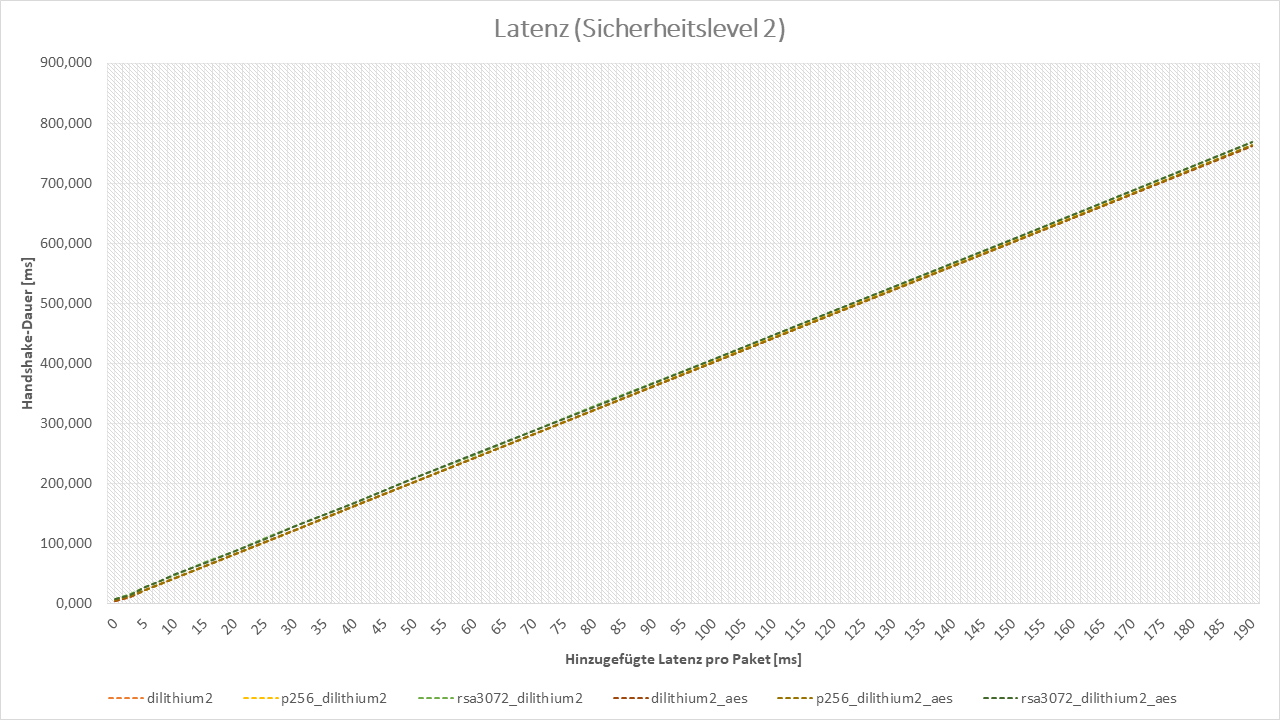
\includegraphics[width=\textwidth]{../auswertung/latenz_sl2.png}
			\caption{Auswertung der Variation der Latenz bei Algorithmen mit Sicherheitslevel 2}
			\label{fig:ergebnis:latenz:sl2}
		\end{figure}
		
		Auch hier kann beobachtet werden, dass Dilithium-2 sowohol mit RSA-3.072 und AES sowie nur mit 					RSA-3.072 eine etwas schlechtere Performanz aufweisen als andere betrachtete Varianten. Jedoch sind die 		Unterschiede auch in diesem Fall so gering, dass sie in der Praxis kaum eine Rolle spielen.\\
		
		Zwischen den Algorithmen der ersten und der zweiten Sicherheitsstufe kann nur ein geringer Unterschied 			in der Performanz beobachtet werden. Bei den Algorithmen der ersten Sicherheitsstufe hatte Falcon-512 				mit RSA-3.072 bei einer hinzugefügten Performanz pro Paket von 190ms mit 767,868 ms die höchste 					Handshake-Dauer.\\
		
		In der zweiten Sicherheitsstufe war dies Dilithium-2, ebenfalls mit RSA-3.072, mit einer maximalen 				Handshake-Dauer von 768,149 ms. Auch diese Abweichung dürfte in der Praxis nicht von Relevanz sein.\\
		
		Für die Praxis kann demnach kein relevanter Performanznachteil der Algorithmen der zweiten 						Sicherheitsstufe gegenüber der ersten festgestellt werden.
		
		\subsection{Sicherheitslevel 3}
		\label{subsec:ergebnis:latenz:sl3}
		
		Auch bei den Algorithmen der dritten Sicherheitsstufe kann der in den Abschnitten 									\ref{subsec:ergebnis:latenz:sl1} und \ref{fig:ergebnis:latenz:sl2} beschriebene Zusammenhang beobachtet 		werden (vgl. Abbildung \ref{fig:ergebnis:latenz:sl3}). Auch hier kann beobachtet werden, dass die 					Performanz der Algorithmen dermaßen nah beieinander liegt, dass sich die Graphen in der Abbildung 					verdecken.
		
		\begin{figure}[htbp]
			\centering
			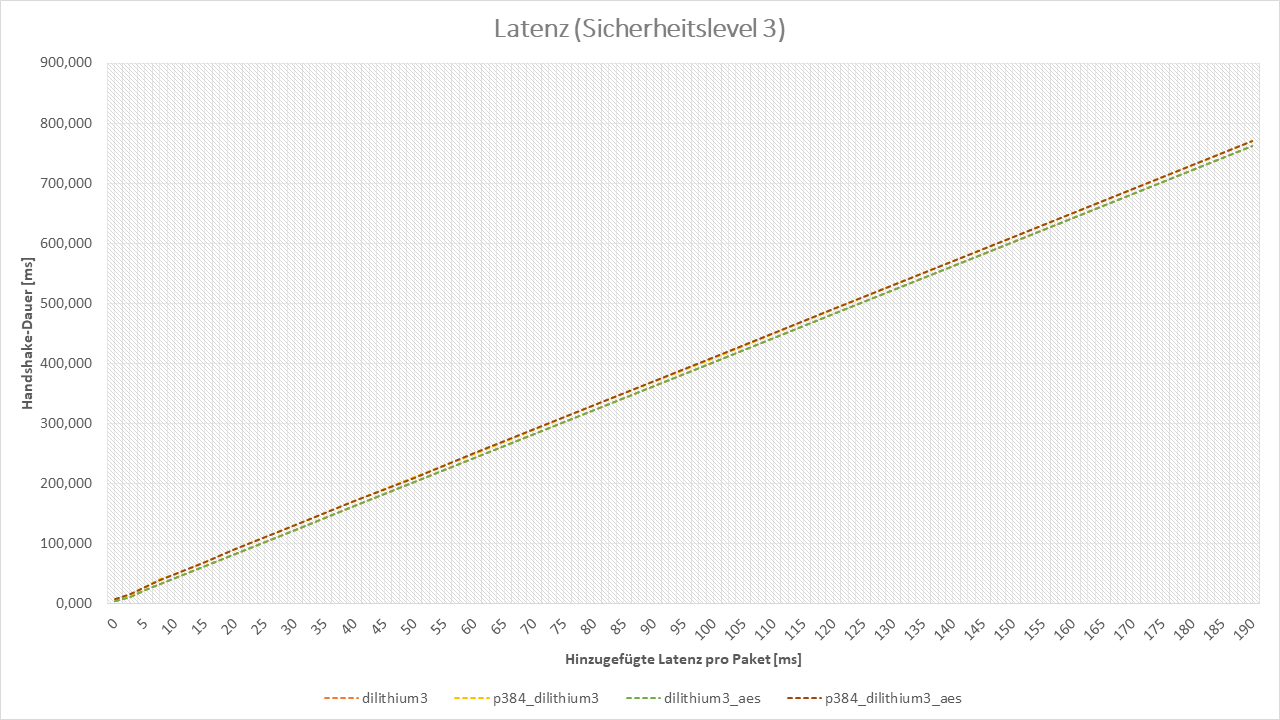
\includegraphics[width=\textwidth]{../auswertung/latenz_sl3.png}
			\caption{Auswertung der Variation der Latenz bei Algorithmen mit Sicherheitslevel 3}
			\label{fig:ergebnis:latenz:sl3}
		\end{figure}
		
		Auch in dieser Gruppe gibt es nur einen sehr geringen Unterschied zwischen dem Algorihmus mit der 					besten und dem Algorithmus mit der schlechtesten Performanz. Am besten performte Dilithium3 mit AES mit 		einer maximalen Handshake-Dauer von 762,213ms. Am schlechtesten schnitt Dilithium-3 mit AES und P-384 				ab. Hier konnte eine maximale Handshake-Dauer von 769,926ms verzeichnet werden.\\
		
		Auch hier sind jedoch die Unterschiede in der Performanz noch sehr gering, sodass für die Praxis kaum 				ein Unterschied festgestellt werden kann.\\
		
		Gegenüber den Algorithmen der niedrigeren Sicherheitsstufen kann auch hier nur ein geringer Nachteil in 		der Performanz festgestellt werden. Sowohl zwischen den Algorithmen der ersten und der zweiten als auch 		zwischen den Algorithmen der zweiten und dritten Sicherheitsstufe kann nur ein Unterschied von rund 1ms 		festgestellt werden.\\
		
		Unter den hier betrachteten Algorithmen wird kein Algorithmus betrachtet, der der Sicherheitsstufe 4 				zuzuordnen ist. Deshalb wird diese im restlichen Verlauf der Arbeit nicht weiter betrachtet.
		
		\subsection{Sicherheitslevel 5}
		\label{subsec:ergebnis:latenz:sl5}
		
		In der fünften Sicherheitsstufe sind zwei verschiedene Algorithmentypen vertreten, die eine deutlich 				unterschiedliche Performanz aufweisen (vgl. Abbildung \ref{fig:ergebnis:latenz:sl5}). Der generelle 				linare Zusammenhang, der in den Abschnitten \ref{subsec:ergebnis:latenz:sl1} bis 									\ref{subsec:ergebnis:latenz:sl3} festgestellt wurde, kann auch hier bestätigt werden.
		
		\begin{figure}[htbp]
			\centering
			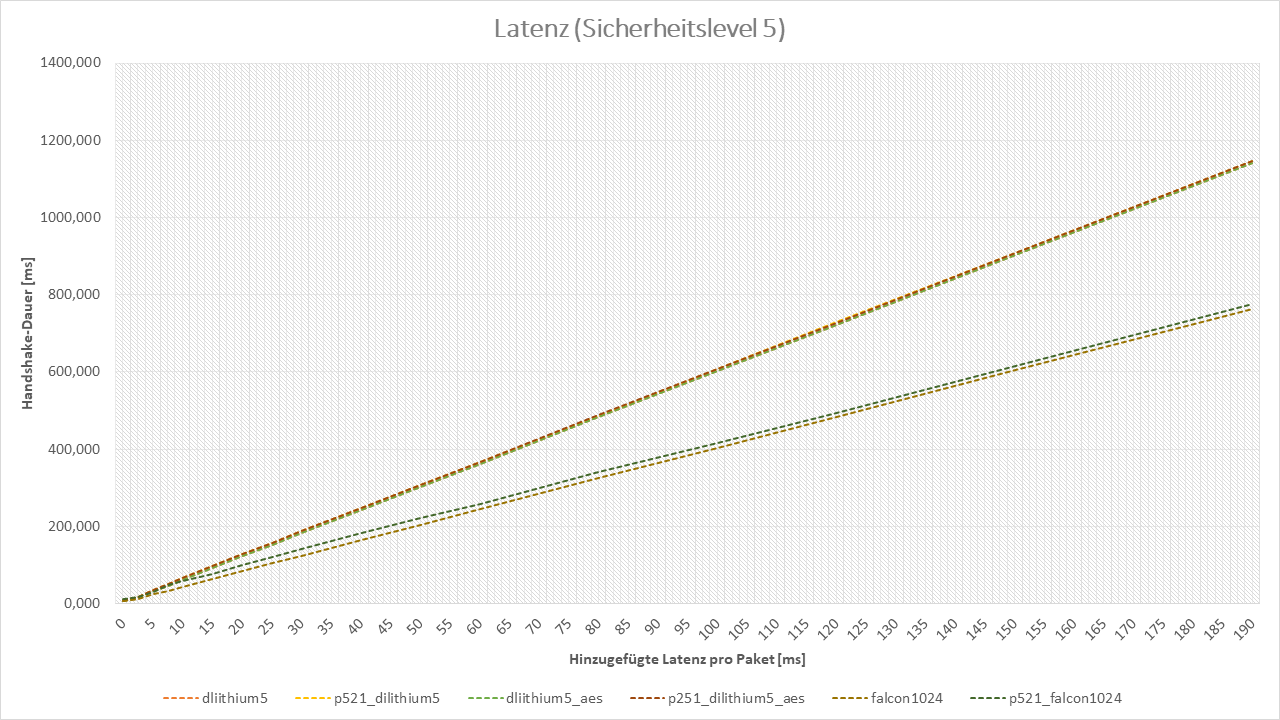
\includegraphics[width=\textwidth]{../auswertung/latenz_sl5.png}
			\caption{Auswertung der Variation der Latenz bei Algorithmen mit Sicherheitslevel 5}
			\label{fig:ergebnis:latenz:sl5}
		\end{figure}
		
		Auffällig ist hier jedoch, dass der geringe Performanz-Unterschied zwischen den geringeren 						Sicherheitsstufen hier bei den 				Dilithium-5-Varianten deutlich stärker vorhanden ist. Bei einer 					hinzugefügten Latenz von 190ms pro Paket ist hier eine maximale 				Handshake-Dauer von 1.147,143ms 					verzeichnet. Dies ist ein signifikanter Performanz-Nachteil gegenüber den Algorithmen der niedrigeren 				Sicherheitsstufen, die maximale Handshake-Dauern im Bereich von 767,868ms bis 769,926ms 				aufweisen.\\
		
		Die Falcon-Varianten hingegen bewegen sich wieder in den aus den niedrigeren Sicherheitsleveln bekannten Bereichen. Der Höchstwert der maximalen Handshake-Dauer liegt auch hier bei 775,923ms. Dies ist erneut eine leicht schlechtere Performanz als in den niedrigeren Sicherheitsleveln. Auch hier handelt es sich jedoch nur um eine geringe Abweichung.\\
		
		An dieser Stelle kann festgelegt werden, dass die Auswahl des eingesetzten Algorithmus für eine Verbindung, die lediglich eine hohe Latenz aufweist, in den meisten Fällen keine besonders große Bedeutung für die Handshake-Dauer in der Praxis hat. Die einzige Ausnahme sind die Dilithium-5-Varianten. Diese weisen mit steigender Latenz eine signifikant höhere Handshake-Dauer auf.
		
	\section{Paketverlust}
	\label{sec:ergebnis:verlust}
	
		\subsection{Sicherheitslevel 1}
		\label{subsec:ergebnis:verlust:sl1}
		
		Im Gegensatz zur Latenz (vgl. Abschnitt \ref{sec:ergebnis:latenz}) ist beim Paketverlust kein klarer linearer Zusammenhang zu erkennen (vgl. 					Abbildung \ref{fig:ergebnis:verlust:sl1}. Es ist zwar klar festzustellen, dass ein höherer Paketverlust mit einer höheren Handshake-Dauer 						einhergeht, es gibt jedoch immer wieder Spitzen im Diagramm.\\
		
		\begin{figure}[htbp]
			\centering
			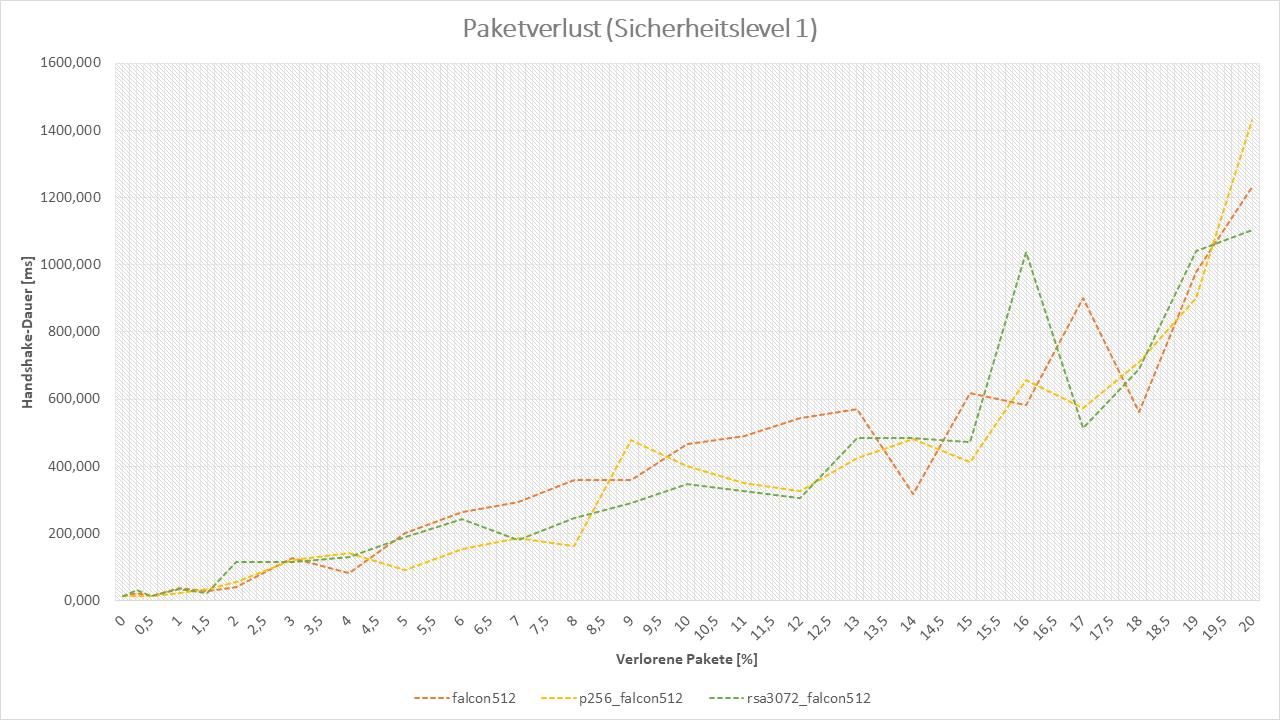
\includegraphics[width=\textwidth]{../auswertung/verlust_sl1.png}
			\caption{Auswertung der Variation des Paketverlusts bei Algorithmen mit Sicherheitslevel 1}
			\label{fig:ergebnis:verlust:sl1}
		\end{figure}
		
		Diese könnten möglicherweise auf das Protokoll TCP zurückzuführen sein. Wenn während der Übertragung, wie hier durch das Testszenario herbeigeführt, 		Pakete verloren gehen, ist TCP dafür zuständig, diese erneut zu senden \cite{Henrich2022}. In diesem Bereich sind weitere Arbeiten notwendig, um das 		beobachtete Phänomen genauer erklären zu können.\\
		
		Auffällig ist an dieser Stelle auch, dass die unterschiedlichen Varianten des betrachteten Algorithmus je nach Rate des Paketverlusts 							unterschiedlich gut performen. Aufgrund der großen beobachteten Spitzen gibt es hier immer wieder Algorithmen, die eine ungewöhnlich hohe Handshake-			Dauer aufweisen, die bei einem höheren Anteil an Paketverlust jedoch wieder geringer wird.\\
		
		Insgesamt schneidet Falcon-512 mit P-256 hier in den betrachteten Bereichen etwas besser ab als die beiden anderen Algorithmen.
		
		\subsection{Sicherheitslevel 2}
		\label{subsec:ergebnis:verlust:sl2}
		
		Im zweiten Sicherheitslevel kann eine besonders signifikante Spitze beim Einsatz von Dilithium-2 mit P-256 beobachtet werden (vgl. Abbildung 					\ref{fig:ergebnis:verlust:sl2}).
		
		\begin{figure}[htbp]
			\centering
			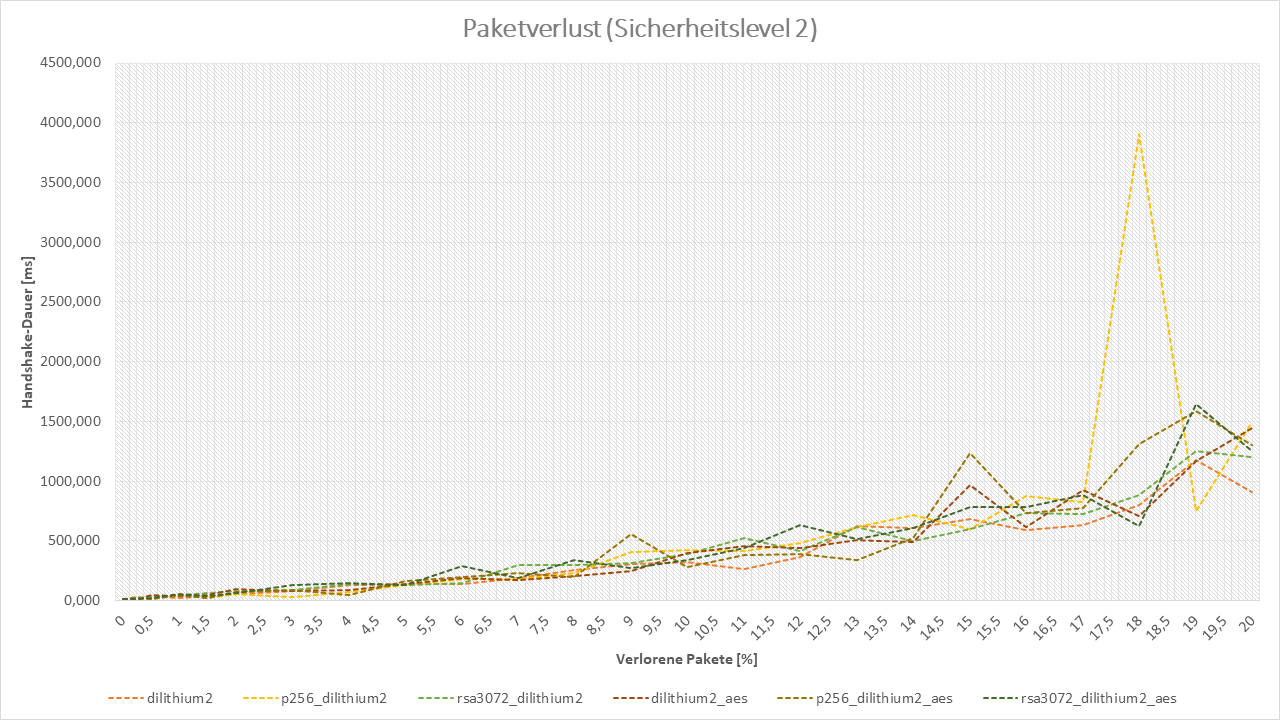
\includegraphics[width=\textwidth]{../auswertung/verlust_sl2.png}
			\caption{Auswertung der Variation des Paketverlusts bei Algorithmen mit Sicherheitslevel 2}
			\label{fig:ergebnis:verlust:sl2}
		\end{figure}
		
		Gerade an dieser Stelle wäre es interessant, in einer zukünftigen Arbeit zu prüfen, ob dieses Verhalten reproduziert werden kann und wodurch dieses 			zustande kommt. Ebenfalls spannend wäre es, zu prüfen, ob solche extremen Spitzen auch in anderen Messbereichen auftreten können. Ein dermaßen 					variables Verhalten ist in der Praxis nicht unbedingt wünschenswert.\\
		
		Weiterhin ist zu beobachten, dass die meisten betrachteten Algorithmen bei dem höchsten getesteten Anteil an verlorenen Paketen von 20\% eine 					Handshake-Dauer im Bereich von 1.200,042ms (Dilithium-2 mit RSA-3.072) bis 1.491,643ms (Dilithium-2 mit P-256) aufweisen. Der einzige Ausreißer 				unter den betrachteten Algorithmen ist Dilithium-2 mit einer Handshake-Dauer von 912,227ms in diesem Bereich.\\
		
		Alle Algorithmen des ersten Sicherheitslevels lagen bei einer Verlustrate von 20\% bei einer maximalen Handshake-Dauer von 1.102,702ms (Falcon-512 				mit RSA-3.072) bis 1.430,114ms (Falcon-512 mit P-256). Auch hier ist kein signifikanter Nachteil in der Performanz durch das Steigen des 						Sicherheitslevels zu beobachten. Einzige Ausnahme ist die beobachtete signifikante Spitze bei Dilithium-2 mit P-256).\\
		
		In den ersten beiden Sicherheitsleveln scheint es, als hätten die Varianten, die P-256 verwenden, einen leichten Vorteil in der Performanz. Hier 				bleibt jedoch zu beobachten, wie hier die starken Spitzen zustande kommen.
		
		\subsection{Sicherheitslevel 3}
		\label{subsec:ergebnis:verlust:sl3}
		
		Im dritten Sicherheitslevel sind ebenfalls kleinere Spitzen zu beobachten, die jedoch nicht so signifikant sind wie in Abschnitt 								\ref{subsec:ergebnis:verlust:sl2} (vgl. Abbildung \ref{fig:ergebnis:verlust:sl3}).
		
		\begin{figure}[htbp]
			\centering
			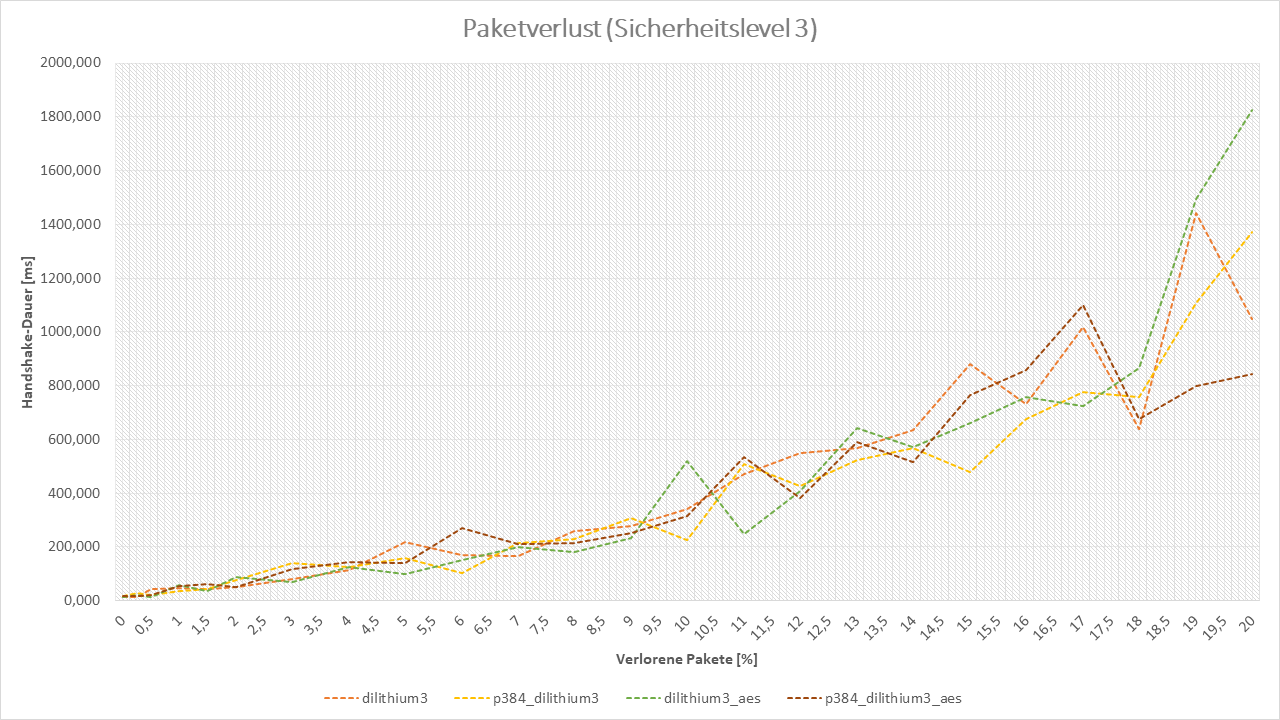
\includegraphics[width=\textwidth]{../auswertung/verlust_sl3.png}
			\caption{Auswertung der Variation des Paketverlusts bei Algorithmen mit Sicherheitslevel 3}
			\label{fig:ergebnis:verlust:sl3}
		\end{figure}
		
		Auffällig ist hier, dass in den Bereichen höherer Paketverluste (ab ca. 18\% eine deutlich stärkere Streuung der Performanz der verschiedenen 					Algorithmen zu beobachten ist.\\
		
		Bei einem maximalen betrachteten Paketverlust von 20\% weist Dilithium-3 mit P-384 und AES mit nur 842,580ms die 				geringste Handshake-Dauer auf. Dilithium-3 mit AES hingegen hat eine Handshake-Dauer von 1.823,656ms. Eine dermaßen große Spanne konnte in keinem 				der beiden unteren Sicherheitsleveln beobachtet werden.\\
		
		Bei einem Paketverlust im Bereich von 17\% bis 18\% bei dem im Sicherheitslevel 2 eine signifikante Spitze bei Dilithium-2 mit P-256 beobachtet 				werden konnte, ist auch hier eine besonders starke Dynamik der gemessenen Werte zu verzeichnen.\\
		
		Besonders stark ausgeprägt ist dies bei Dilithium-3 und Dilithium-3 mit P-384 und AES. In einer weiteren Arbeit wäre es interessant, zu prüfen, 				inwiefern die Verwendung der elliptischen Kurven an dieser Stelle die Performanz begünstigt und warum hier besonders variable Messwerte beobachtet 				werden.
		
		\subsection{Sicherheitslevel 5}
		\label{subsec:ergebnis:verlust:sl5}
		
		Im fünften Sicherheitslevel können die in den vorherigen Sicherheitsstufen betrachteten Beobachtungen bestätigt werden (vgl. Abbildung 							\ref{fig:ergebnis:verlust:sl5}). Es können sowohl einige Spitzen beobachtet werden als auch eine im Vergleich zu den niedrigeren Sicherheitsstufen 				größere Streuung der Handshake-Dauern der Algorithmen bei den höheren betrachteten Verlustraten.
		
		\begin{figure}[htbp]
			\centering
			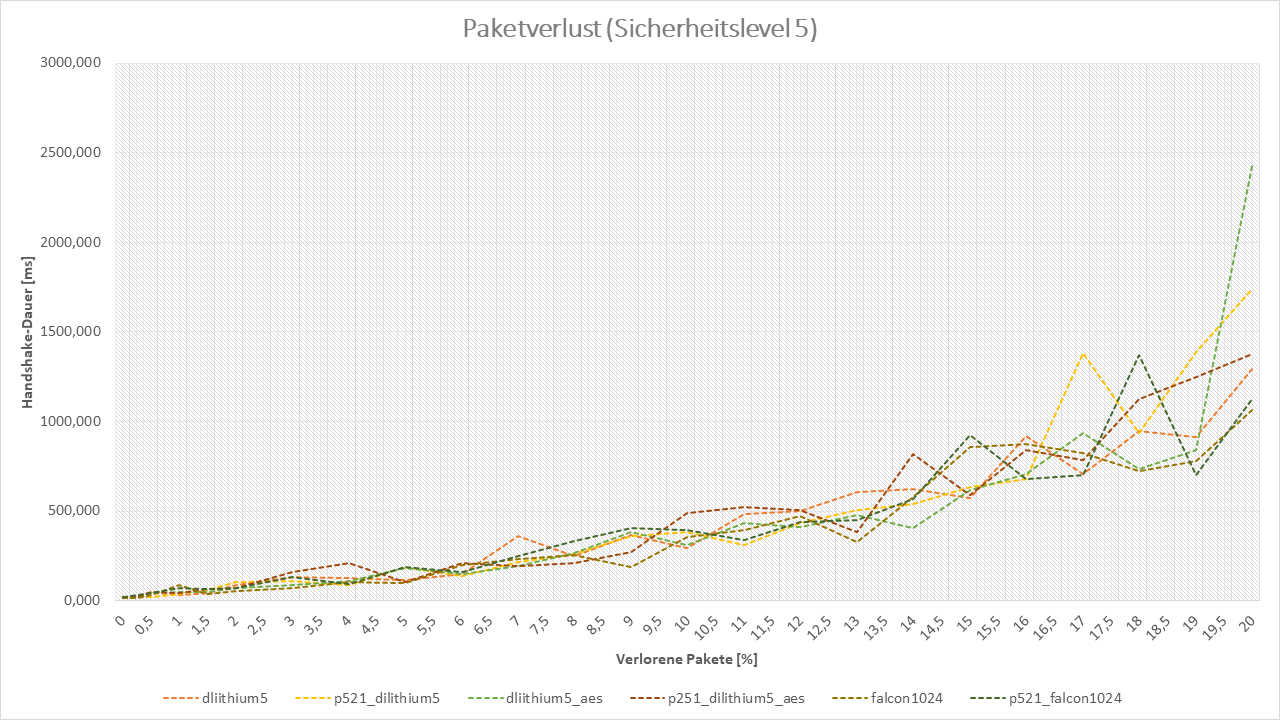
\includegraphics[width=\textwidth]{../auswertung/verlust_sl5.png}
			\caption{Auswertung der Variation des Paketverlusts bei Algorithmen mit Sicherheitslevel 5}
			\label{fig:ergebnis:verlust:sl5}
		\end{figure}
		
		Auch hier sind im Bereich der Verlustraten von ca. 17\% bis 19\% deutliche Spitzen bei den Algorithmen Dilithium-5 mit P-521 und Falcon-1.024 mit 				P-521 zu erkennen. Dass dies bei beiden Algorithmengruppen auftritt, deutet ebenfalls darauf hin, dass diese Spitzen mit der verwendung der 					elliptischen Kurven zusammenhängt.\\
		
		Ebenfalls bestätigt werden kann die große Streuung der Handshake-Dauern. Bei einer Verlustrate von 20\% hat Falcon-1.024 mit 1.065,197ms die 					geringste Handshake-Dauer. Die höchste Handshake-Dauer kann bei Dilithium-5 mit AES beobachtet werden. Diese beträgt mit 2.428,096ms deutlich mehr 				als das Doppelte.\\
		
		Um hier eine klare Empfehlung aussprechen zu können, bedarf es weiterer Forschung (vgl. Kapitel \ref{ch:reflexion}). Es scheint jedoch, als hätten 				die Algorithmen, die elliptische Kurven nutzen einen Performanz-Vorteil.
		
	\section{Doppelte Pakete}
	\label{sec:ergebnis:doppelt}
	
		\subsection{Sicherheitslevel 1}
		\label{subsec:ergebnis:doppelt:sl1}
		
		Doppelte Pakete scheinen keine bedeutende Auswirkung auf die Performanz der betrachteten Algorithmen zu haben. Es kann kein genereller Anstieg 					beobachtet werden (vgl. Abbildung \ref{fig:ergebnis:doppelt:sl1}).
		
		\begin{figure}[htbp]
			\centering
			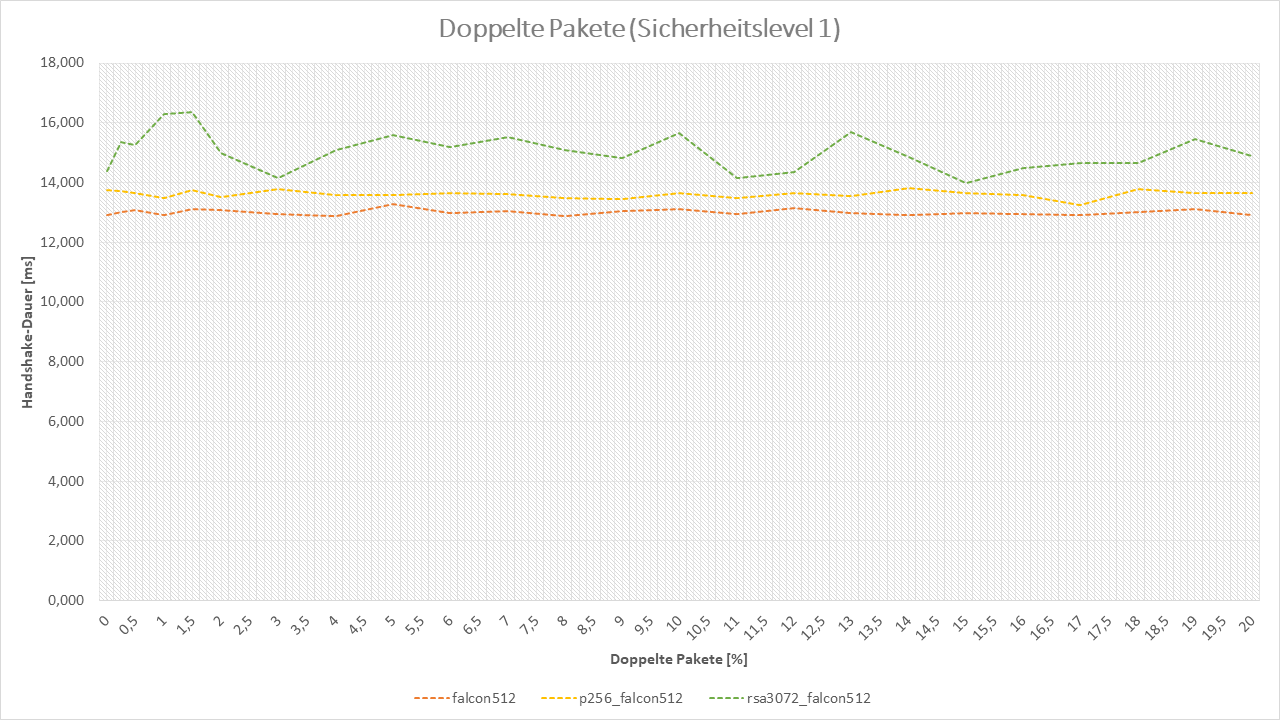
\includegraphics[width=\textwidth]{../auswertung/doppelt_sl1.png}
			\caption{Auswertung der Variation doppelter Pakete bei Algorithmen mit Sicherheitslevel 1}
			\label{fig:ergebnis:doppelt:sl1}
		\end{figure}
		
		Zunächst fällt auf, dass die Spanne der Ergebnisse für jeden der betrachteten Algorithmen so gering ist, dass sich die Graphen in der Abbildung an 				keiner Stelle überschneiden.\\
		
		Auffällig ist ausßerdem, dass das reine Falcon-512 hier in allen betrachteten Messreihen die geringste Handshake-Dauer und somit die beste 						Performanz vorweisen kann.\\
		
		Es konnten Handshake-Dauern im Bereich von 12,874ms bis 13,269ms beobachtet werden. Dies ist im Vergleich zu den in den 				Abschnitten \ref{sec:ergebnis:latenz} und \ref{sec:ergebnis:verlust} beobachteten Spannen eine sehr geringe Abweichung.\\
		
		Die höchsten Werte konnte bei Falcon-512 mit RSA-3.072 verzeichnet werden. Hier besteht mit einem Bereich von 13,986ms bis 16,359ms auch eine 					deutlich größere Spanne als bei den anderen beiden Algorithmen.
		
		\subsection{Sicherheitslevel 2}
		\label{subsec:ergebnis:doppelt:sl2}
		
		In der zweiten Sicherheitsstufe werden etwas mehr Algorithmen betrachtet als in der ersten Sicherheitsstufe, sodass es hier trotz ebenfalls geringer 		Spannen bei den Messwerten pro Algorithmus zu einigen Überschneidungen kommt (vgl. Abbildung \ref{fig:ergebnis:doppelt:sl2}).
		
		\begin{figure}[htbp]
			\centering
			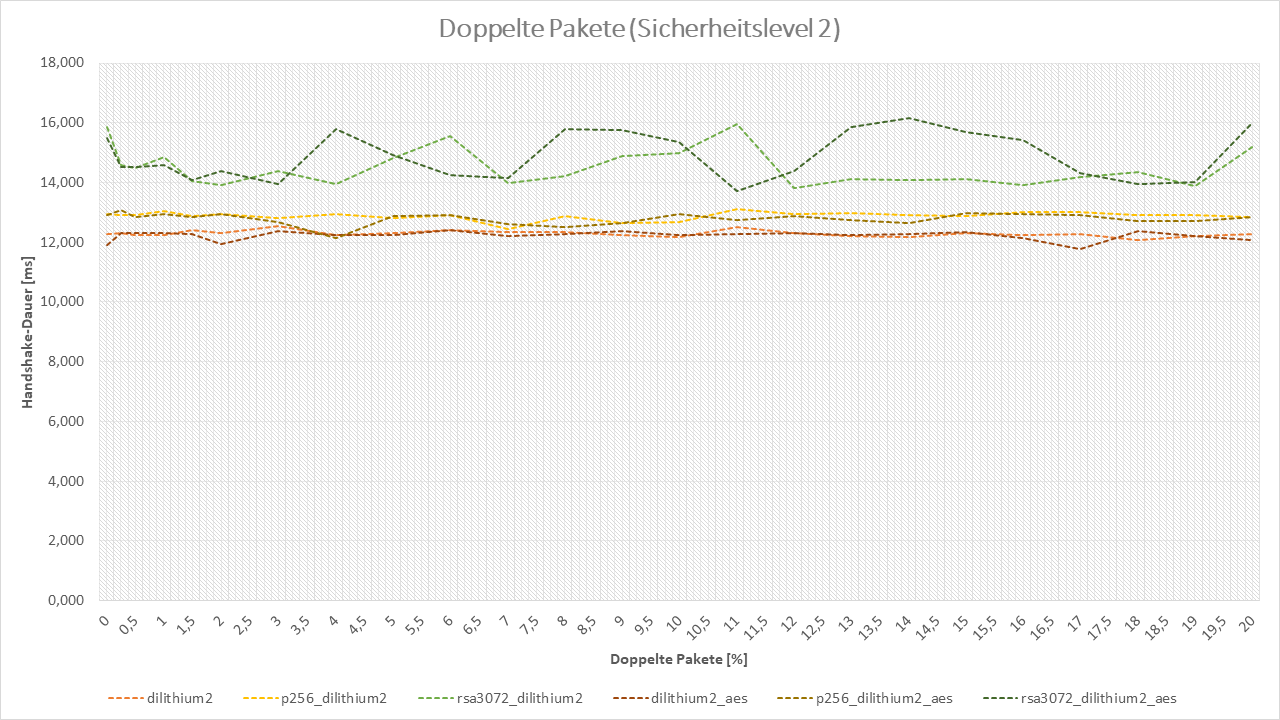
\includegraphics[width=\textwidth]{../auswertung/doppelt_sl2.png}
			\caption{Auswertung der Variation doppelter Pakete bei Algorithmen mit Sicherheitslevel 2}
			\label{fig:ergebnis:doppelt:sl2}
		\end{figure}
		
		Die Beobachtung aus dem ersten Sicherheitslevel, dass die Algorithmusvarianten, die RSA-3.072 verwenden, die höchste Handshake-Dauer aufweisen, kann auch hier deutlich bestätigt werden.\\
		
		Für Dilithium-2 mit RSA-3.072 konnte eine Handshake-Dauer im Bereich von 13,802ms bis 15,943ms aufgezeichnet werden. Für Dilithium-2 mit RSA-3.072 und AES wurde eine Handshake-Dauer von 13,711ms bis 16,168ms beobachtet.\\
		
		Dies entspricht nicht nur einer deutlich höheren Handshake-Dauer im Vergleich zu den anderen betrachteten Algorithmen, die sich insgesamt in einem Bereich von 11,782ms bis 13,115ms bewegen, sondern auch einer deutlich höheren Streuung (vgl. Abbildung \ref{fig:ergebnis:doppelt:sl2}).\\
		
		Betrachtet man die restlichen Algorithmen genauer, scheinen Varianten, die elliptische Kurven verwenden, einen geringen Performanz-Nachteil zu haben. Dilithium-2 mit P-256 hat Handshake-Dauern im Bereich von 12,445ms bis 13,115ms, während reines Dilithium-2 eine Spanne von 12,063ms bis 12,540ms abdeckt.\\
		
		Genauso hat Dilithium-2 mit AES und P-256 Handshake-Dauern von 12,138ms bis 12,980ms. Dilithium-2 mit AES hingegen bewegt sich zwischen 11,782ms und 12,399ms.
		
		\subsection{Sicherheitslevel 3}
		\label{subsec:ergebnis:doppelt:sl3}
		
Im dritten Sicherheitslevel können die Beobachtungen aus den ersten beiden Sicherheitsleveln weitestgehend bestätigt werden (vgl. Abbildung \ref{fig:ergebnis:doppelt:sl3}).		
		
		\begin{figure}[htbp]
			\centering
			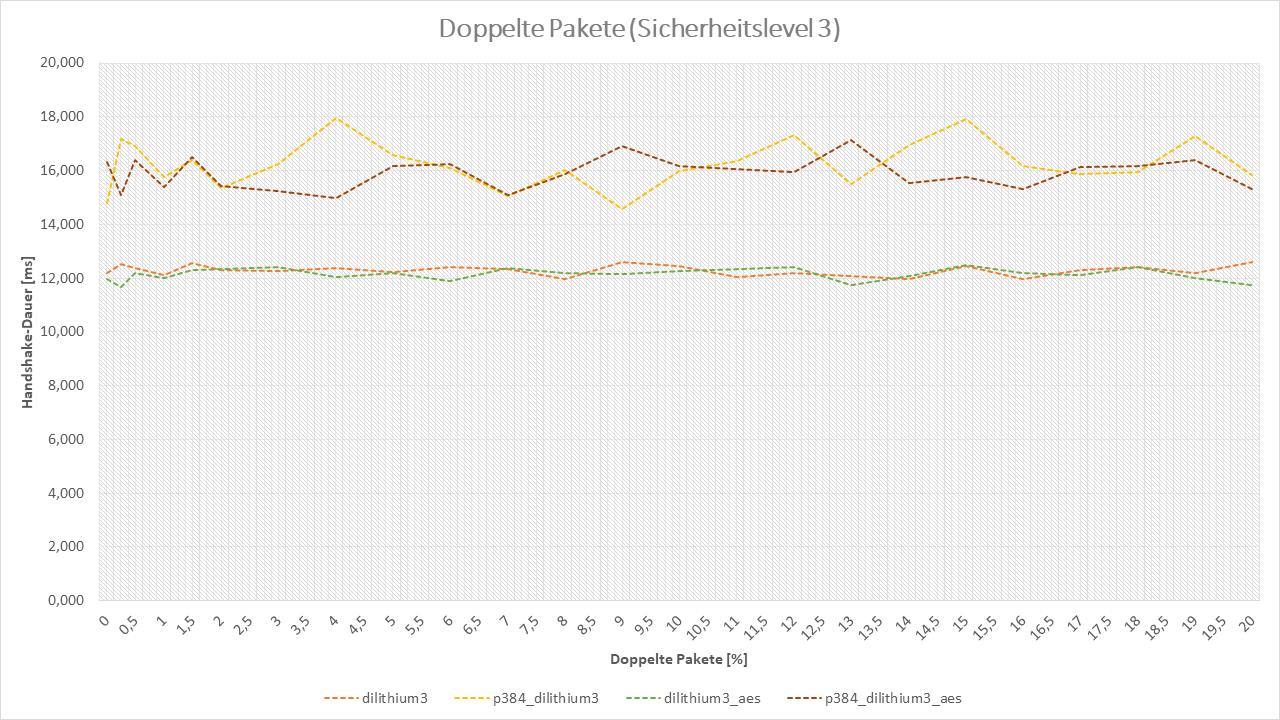
\includegraphics[width=\textwidth]{../auswertung/doppelt_sl3.png}
			\caption{Auswertung der Variation doppelter Pakete bei Algorithmen mit Sicherheitslevel 3}
			\label{fig:ergebnis:doppelt:sl3}
		\end{figure}
		
		In dieser Gruppe waren keine Algorithmen, die RSA verwenden, vertreten. Somit konnte die Vermutung aus Abschnitt \ref{subsec:ergebnis:doppelt:sl2}, dass diese Algorithmen eine höhere Handshake-Dauer sowie eine höhere Dynamik in den gemessenen Handshake-Dauern aufweisen, hier nicht weiter betrachtet werden.\\
		
		Allerdings fällt auch hier auf, dass die Varianten, die elliptische Kurven verwenden, einen geringen Performanz-Nachteil gegenüber den Varianten haben, die dies nicht tun.\\
		
		Dilithium-3 mit P-384 weist Handshake-Dauern zwischen 14,575ms und 17,943ms auf, während reines Dilithium-3 eine Spanne von 11,965ms bis 12,604ms hat. Analog dazu hat Dilithium-3 mit AES und P-384 Handshake-Dauern von 14,992ms bis 17,121ms, während sich Dilithium-3 mit AES von 11,682ms bis 12,480ms bewegt.\\
		
		Dies entspricht nicht nur höheren Handshake-Dauern bei den Varianten, die elliptische Kurven verwenden. Zu beobachten ist auch, eine größere Spanne, die in Abbildung \ref{fig:ergebnis:doppelt:sl3} ebenfalls gut erkennbar ist.
		
		\newpage
		
		\subsection{Sicherheitslevel 5}
		\label{subsec:ergebnis:doppelt:sl5}
		
Auch in der letzten betrachteten Sicherheitsstufe können die in den Abschnitten \ref{subsec:ergebnis:doppelt:sl1} bis \ref{subsec:ergebnis:doppelt:sl3} gemachten Beobachtungen bestätigt werden (vgl. Abbildung \ref{fig:ergebnis:doppelt:sl5}).		
		
		\begin{figure}[htbp]
			\centering
			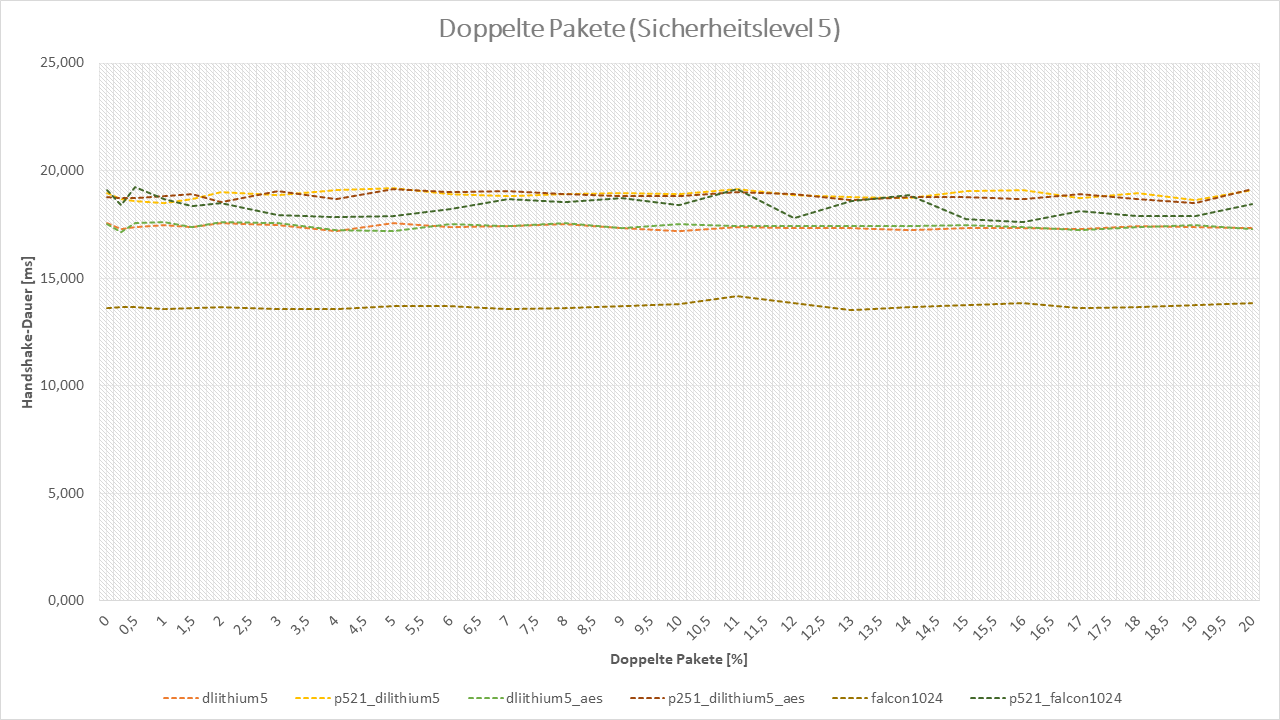
\includegraphics[width=\textwidth]{../auswertung/doppelt_sl5.png}
			\caption{Auswertung der Variation doppelter Pakete bei Algorithmen mit Sicherheitslevel 5}
			\label{fig:ergebnis:doppelt:sl5}
		\end{figure}
		
		Auch in dieser Gruppe sind keine Varianten vertreten, die RSA verwenden, sodass die Beobachtung aus Abschnitt \ref{subsec:ergebnis:doppelt:sl2} nicht weiter geprüft werden kann.\\
		
		Es kann jedoch auch hier beobachtet werden, dass die Algorithmen, die elliptische Kurven verwenden, eine höhere Handshake-Dauer sowie eine größere Spanne der Messwerte aufweisen. Dilithium-5 mit P-521 hat Handshake-Dauern von 18,476ms bis 19,119ms, während sich Dilithium-5 in einem Bereich von 17,167ms bis 17,553ms bewegt.\\
		
		Analog dazu hat Dilithium-5 mit AES und P-521 Handshake-Dauern von 18,506ms bis 19,145ms, während Dilithium-5 mit AES eine Spanne von 17,140ms bis 17,598ms aufweist.\\
		
		Besonders auffällig ist dieses Verhältnis bei Falcon-1.024. Hier konnten bei Verwendung von P-521 Handshake-Dauern von 17,614ms bis 19,227ms aufgezeichnet werden. Dies entspricht etwa den Ergebnissen der anderen Algorithmen. Bei der Verwendung von reinem Falcon-1.024 lagen die Messwerte jedoch zwischen 13,510ms und 14,184ms, was einer vergleichsweise sehr geringen Handshake-Dauer entspricht.
		
	\section{Begrenzte Bandbreite}
	\label{sec:ergebnis:bandbreite}
	
		\subsection{Sicherheitslevel 1}
		\label{subsec:ergebnis:bandbreite:sl1}
		
		Der signifikanteste Zusammenhang zwischen einer Veränderung der Netzwerkparameter und der Dauer des Handshakes konnte bei der Begrenzung der Bandbreite beobachtet werden. Eine zunehmende Begrenzung der Bandbreite verursachte ein exponenzielles Wachstum der Handshake-Dauer (vgl. Abbildung \ref{fig:ergebnis:bandbreite:sl1}.
		
		\begin{figure}[htbp]
			\centering
			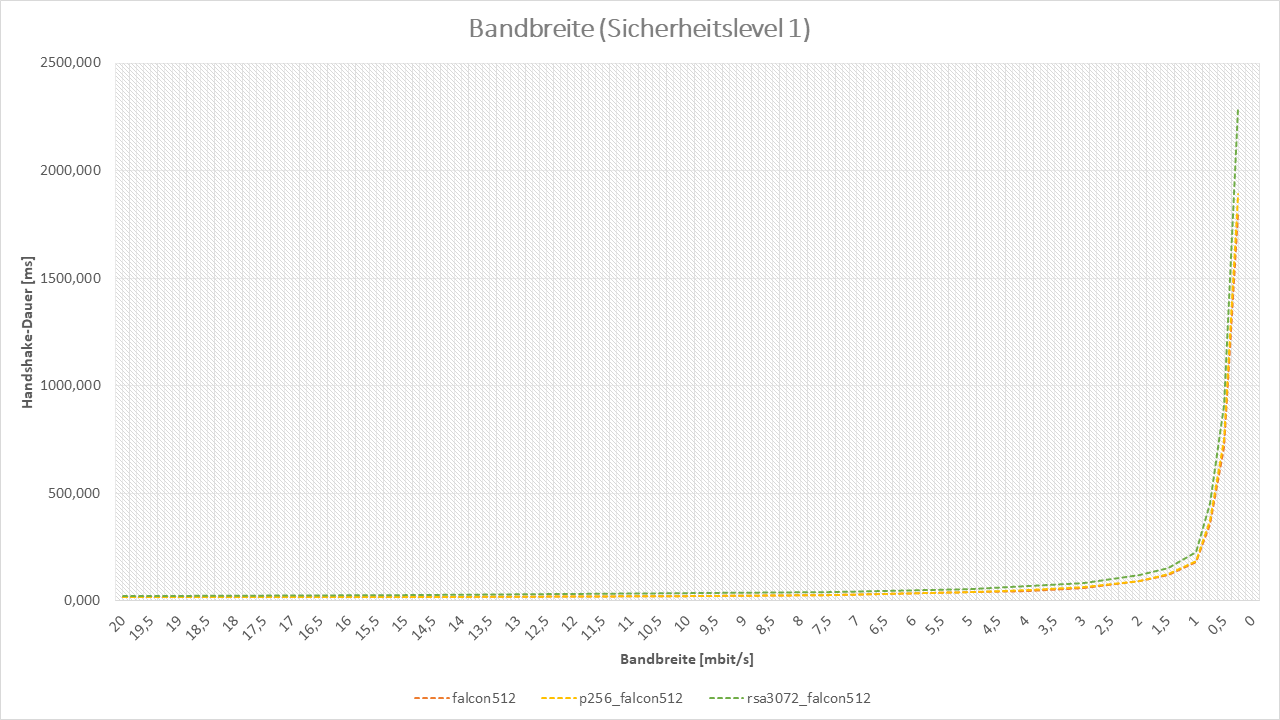
\includegraphics[width=\textwidth]{../auswertung/bandbreite_sl1.png}
			\caption{Auswertung der Variation der Bandbreite bei Algorithmen mit Sicherheitslevel 1}
			\label{fig:ergebnis:bandbreite:sl1}
		\end{figure}
		
		Ein starker Anstieg der Handshake-Dauer kann dabei ab einer Begrenzung der Bandbreite auf ca. 1mbit/s beobachtet werden.\\
		
		Der beobachtete Unterschied zwischen Falcon-512 und Falcon-512 mit P-256 ist dabei so gering, dass die Graphen einander in der Abbildung teils überdecken.\\
		
		Falcon-512 mit RSA-3.072 scheint einen geringen Nachteil in der Performanz zu haben. Dieser sollte in der Praxis jedoch in Anbetracht des allgemeinen exponenziellen Wachstums eine untergeordnete Rolle spielen.
		
		\subsection{Sicherheitslevel 2}
		\label{subsec:ergebnis:bandbreite:sl2}
		
		Auch in der zweiten Sicherheitsstufe kann ein exponenzielles Wachstum der Handshake-Dauer beobachtet werden (vgl. Abbildung \ref{fig:ergebnis:bandbreite:sl2}).\\
		
		\begin{figure}[htbp]
			\centering
			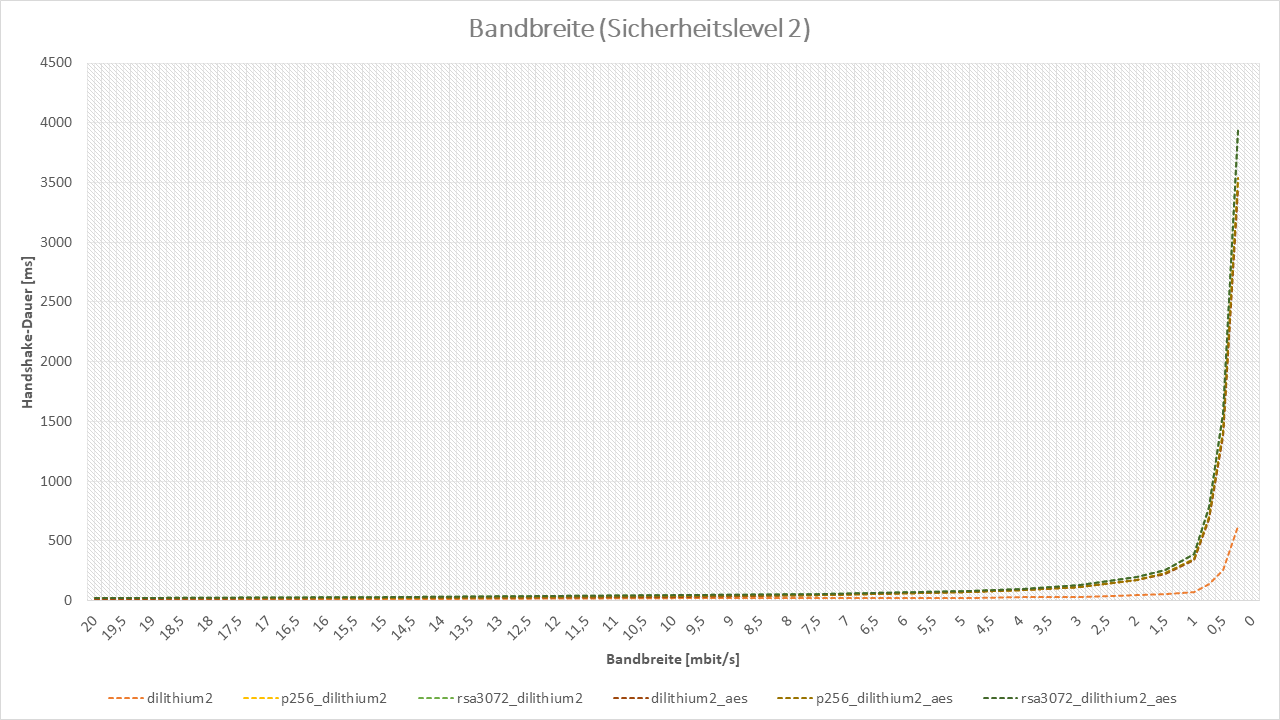
\includegraphics[width=\textwidth]{../auswertung/bandbreite_sl2.png}
			\caption{Auswertung der Variation der Bandbreite bei Algorithmen mit Sicherheitslevel 2}
			\label{fig:ergebnis:bandbreite:sl2}
		\end{figure}
		
		Hier ist jedoch deutlich hervorzuheben, dass Dilithium-2 auch bei geringeren zur Verfügung stehenden Bandbreiten eine deutlich geringere Handshake-Dauer aufweist als die anderen betrachteten Algorithmen.
		
		\subsection{Sicherheitslevel 3}
		\label{subsec:ergebnis:bandbreite:sl3}
		
		Im dritten Sicherheitslevel liegen die Messwerte der betrachteten Algorithmen so eng beieinander, dass praktisch kein Unterschied erkennbar ist (vgl. Abbildung \ref{fig:ergebnis:bandbreite:sl3}).
		
		\begin{figure}[htbp]
			\centering
			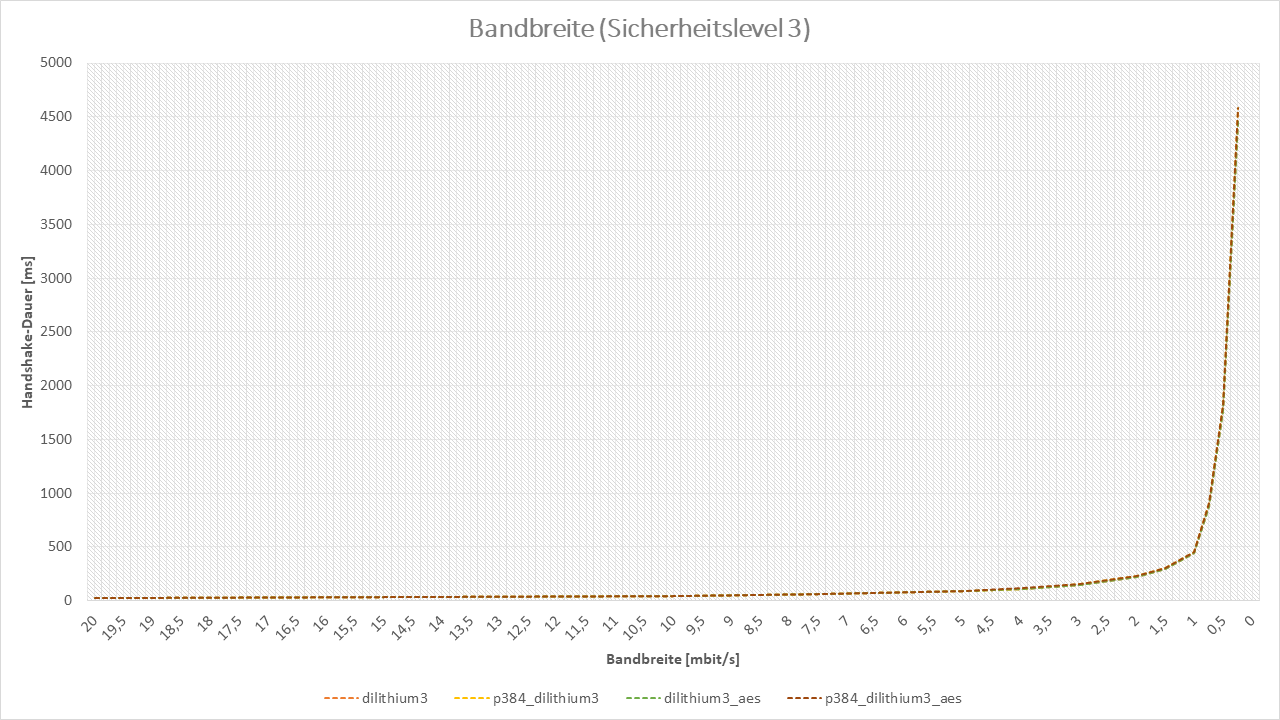
\includegraphics[width=\textwidth]{../auswertung/bandbreite_sl3.png}
			\caption{Auswertung der Variation der Bandbreite bei Algorithmen mit Sicherheitslevel 3}
			\label{fig:ergebnis:bandbreite:sl3}
		\end{figure}
		
		\subsection{Sicherheitslevel 5}
		\label{subsec:ergebnis:bandbreite:sl5}
		
		Im letzten betrachteten Sicherheitslevel sind zwei distinktiv unterschiedliche Gruppen an Algorithmen zu beobachten (vgl. Abbildung \ref{fig:ergebnis:bandbreite:sl5}).
		
		\begin{figure}[htbp]
			\centering
			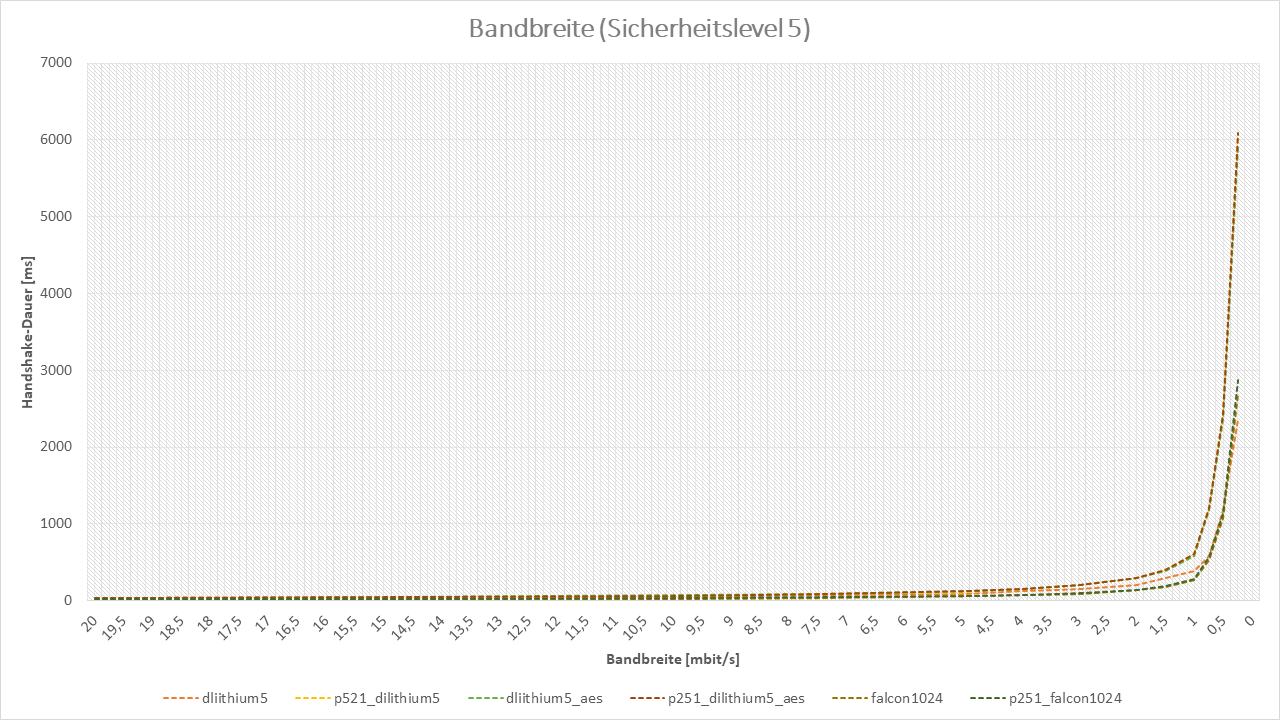
\includegraphics[width=\textwidth]{../auswertung/bandbreite_sl5.png}
			\caption{Auswertung der Variation der Bandbreite bei Algorithmen mit Sicherheitslevel 5}
			\label{fig:ergebnis:bandbreite:sl5}
		\end{figure}
		
		Bei der letzten betrachteten Messung mit einer Bandbreite von 0,25mbit/s konnte Dilithium-5 eine Handshake-Dauer von 2.370,467ms aufweisen. Sowohl Dilithium-5 mit P-521 als auch Dilithium-5 mit AES und Dilithium-5 mit P-521 und AES bewegen sich hingegen in einem deutlich höheren Bereich von 5.914,076ms bis 6085,405ms. Dies scheint die Beobachtung aus Abschnitt \ref{subsec:ergebnis:bandbreite:sl2} zu bestätigen.\\
		
		Bei den Falcon-1.024-Varianten kann hingegen kein dermaßen großer Unterschied festgelegt. Bei einer Begrenzung der Bandbreite auf 0,25mbit/s dauert der Handshake mit Falcon-1.024 2.697,063ms. Bei Verwendung von P-521 steigt dieser Wert nur leicht an auf 2.868,685ms.\\
		
		Insgesamt ist an dieser Stelle aus Sicht der Performanz zu empfehlen, eine reine Dilithium-Variante oder eine Falcon-Variante zu wählen.
